\documentclass[a4paper,11pt]{report}
\usepackage[utf8]{inputenc}
\usepackage{graphicx}
\usepackage{hyperref}
\usepackage{listings}
\usepackage{float}
\hypersetup{
    colorlinks,
    citecolor=black,
    filecolor=black,
    linkcolor=black,
    urlcolor=black
}
\hypersetup{pdfstartview={XYZ null null 1.00}}

\usepackage[nottoc]{tocbibind}

\graphicspath{{img/}} % Ruta donde están las imágenes

% Para que no corte las palabras

\pretolerance=2000
\tolerance=3000

\begin{document}

% Renombramos las figuras y las tablas
\renewcommand{\contentsname}{Índice}
\renewcommand{\chaptername}{Capítulo}
\renewcommand{\figurename}{Figura}
\renewcommand{\listfigurename}{Índice de figuras}
\renewcommand{\tablename}{Tabla}
\renewcommand{\listtablename}{Índice de tablas}
\renewcommand\bibname{Bibliografía}

% Portada
\pagestyle{empty}
\begin{titlepage}

	\begin{figure}[htbp] 
		\centering 
		
\includegraphics[scale=1]{logo_ugr.png}
		\hspace{3.0cm}
		
\includegraphics[scale=0.25]{logo_lsi.png}
	\end{figure}
    
	\begin{center}
	
		\vspace{1.0cm}
		
		\LARGE{\textbf{UNIVERSIDAD DE GRANADA}} \\
		
		\vspace{1.0cm}
		
		\LARGE{\textbf{DEPARTAMENTO DE LENGUAJES Y SISTEMAS INFORMÁTICOS}} \\
		
		\vspace{1.0cm}
		
		\textbf{Escuela Técnica Superior de Ingenierías Informática y Telecomunicaciones} \\
		
		\vspace{1.0cm}
		
		\Large{\textbf{INGENIERÍA INFORMÁTICA}} \\
		
		\vspace{1.0cm}
		
		\Large{PROYECTO FIN DE CARRERA} \\
		
		\vspace{0.5cm}

		\Large{\emph{Traffic Flow Simulator}} \\
		
		\vspace{1.5cm}
		
		\Large{Juan Antonio Fajardo Serrano} \\
		
		\vspace{0.5cm}
		
		\Large{Director del proyecto: Domingo Martín Perandrés} \\
		
		\vspace{0.5cm}
		
		\large{Curso 2014/2015}
		
	\end{center}
\end{titlepage}
\pagebreak
% Inserción de página en blanco
\newpage
\thispagestyle{empty}
\mbox{}
% Fin inserción de página en blanco
\pagestyle{plain}
% Posible inclusión de primera hoja, agradecimientos, licencia,...

\tableofcontents

\chapter{Introducción}
\paragraph{}
La presente memoria documenta el desarrollo de un simulador de tráfico, denominado \emph{Traffic Flow Simulator}, que tendrá como base una interfaz gráfica desde la que el usuario podrá introducir cambios en las variables involucradas en la simulación y ver los resultados que ocasionan.

\paragraph{}
La simulación está definida como una representación de cierta parte del mundo real conseguida mediante la construcción de un modelo de ordenador que va evolucionando a lo largo del tiempo \cite{Drew1968}. Según \emph{Simulation of traffic systems} \cite{Pursula}, el desarrollo de simuladores de tráfico mediante ordenador comenzó en 1955 con la tesis de Daniel L. Gerlough en la Universidad de California. En la actualidad, gracias al poder de cálculo de los computadores, se han logrado grandes avances en este campo, como algunos simuladores a escala macroscópica.

	\begin{figure}[H]
		\centering
			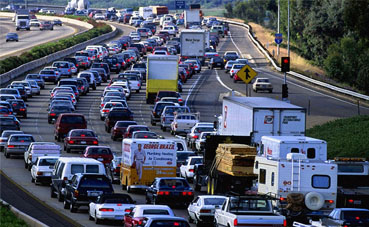
\includegraphics[scale=0.75]{traffic.jpg}
		\caption{Congestión del tráfico.}
		\label{fig:TrafficJam}
	\end{figure}

\paragraph{}
Este proyecto nace del problema actual de tráfico en las grandes ciudades y la necesidad de mejorar el flujo de vehículos en puntos concretos de las zonas urbanas, que es actualmente un problema diario.

\paragraph{}
\emph{Traffic Flow Simulator} tiene como objetivo principal ser una herramienta útil que facilite la visualización de la simulación del tráfico en base a un modelo lógico, de forma que permita evaluar de manera clara las diferentes alternativas a situaciones concretas, permitiendo al usuario recrear dichas situaciones mediante la interacción con la herramienta teniendo en cuenta puntos importantes como son la congestión de las vías o los comportamientos de conducción, de forma que se pueda mejorar el flujo de tráfico en las vías urbanas.

\paragraph{}
El flujo de tráfico de vehículos es un sistema complejo y difícil de modelar y medir, ya que en este se ven involucradas multitud de variables dependientes unas de otras, entre las que destacan los problemas de movilidad, los cambios de sentido, las rotondas, los tiempos de semaforización, las obras en la calzada, los accidentes de tráfico y otras variables sin contar con el factor humano y las condiciones atmosféricas.

\paragraph{}
Este simulador posibilitará realizar simulaciones de tráfico sobre distintas distribuciones de redes viarias, teniendo en cuenta los diferentes perfiles de conductores que podemos encontrarnos día a día en la carretera. Así mismo, el usuario podrá personalizar las distintas variables que influirán en la simulación de forma que pueda recrear los escenarios que desee.

\paragraph{}
La parte visual estará compuesta por un entorno pasivo que no afectará al tráfico y otro activo que afectará directamente al tráfico como son semáforos y vehículos. 


\chapter{Objetivos}
	\paragraph{}
	En este capítulo se mostrarán los objetivos que han sido marcados para la realización de este proyecto.

\section{Objetivo principal del proyecto}

	\paragraph{}
	El objetivo principal de este proyecto es la obtención de una aplicación multiplataforma de código abierto que permita observar, de forma gráfica en tres dimensiones, el flujo de tráfico de vehículos en distintas configuraciones de red viaria, que el usuario podrá cambiar mediante la interacción con la aplicación.
	
\section{Red viaria}

	\paragraph{}
	La red viaria con la que trabajará el simulador será una red sencilla, en la cual, habrá puntos por los que entrarán y saldrán los vehículos hacia y desde la porción de red viaria que se esté simulando, habrá intersecciones de mínimo tres vías y máximo cuatro vías y algún mecanismo que nos permita definir curvas sin realizar intersecciones.

\section{Señales de tráfico}

	\paragraph{}
	Como señales para controlar el flujo de tráfico, la red viaria contará con semáforos en las intersecciones que se encargarán de permitir el paso alternativo de vehículos entre las distintas vías que lleguen a cada una de las intersecciones.
	
\section{Vehículos}
	
	\paragraph{}
	Los vehículos que intervendrán en la simulación serán de al menos tres tipos, coches, autobuses, y camiones no articulados.
	
	\paragraph{}
	Los modelos de estos vehículos serán de poco nivel de detalle con el fin de poder incluir en la simulación tantos como se pueda sin que se vea afectado el rendimiento del sistema.
	
	\paragraph{}
	El usuario podrá variar el número de vehículos involucrados en la simulación así como la proporción del tipo de vehículos (públicos o privados) mediante la interacción con la interfaz gráfica.
	
\section{Conductores}

	\paragraph{}
	Para simular el flujo de tráfico de una forma más realista, el sistema conductista contará con al menos tres tipos de conductores, aquellos que cumplen las normas de circulación siempre, aquellos que las cumplen normalmente y por último, aquellos que casi nunca las cumplen, en menor proporción respecto a los otros dos tipos.
	
	\paragraph{}
	El usuario podrá cambiar la proporción de los tres tipos de conductores mediante la interacción con la interfaz gráfica.
	
\section{Entorno}
	
	\paragraph{}
	El entorno estará formado por los elementos que conforman las vías de la red (plataforma de la vía, líneas de arcenes, líneas de mediana, líneas de carril taxi bus, líneas discontinuas para los carriles normales, y líneas de detención), señales horizontales para indicar carriles normales y carriles taxi bus, túneles para indicar los puntos por los que los vehículos entrarán y saldrán de la porción de red viaria simulada, y semáforos de tres estados para la regulación del tráfico.
	

\chapter{Estado del arte}
	\paragraph{}
	En el presente capítulo se abordará el estado del arte de los distintos elementos de los que se hará uso en el desarrollo de este proyecto.
	
	\paragraph{}
	En el apartado \emph{Simuladores de tráfico} se presentará la esencia del proyecto; en el apartado \emph{Representación de redes viarias}, se tratará una manera de trabajar con los mapas de redes viarias de forma que podamos generar el entorno en el que se desenvolverán los vehículos en nuestro simulador; en el apartado \emph{Sistemas de partículas conductistas} se presentará el modelo de interacción utilizado por los vehículos mencionados anteriormente; en el apartado \emph{Modelos de redes viarias reales a partir de imágenes} abordaremos un método mediante el cual podremos extraer la información de las redes viarias a partir de imágenes; finalmente, en el apartado \emph{Herramientas gráficas} veremos las herramientas que se vienen utilizando para la creación de simuladores de tráfico.

\section{Simuladores de tráfico}

	% ¿Qué es? y ¿Para qué sirve?

	\paragraph{}
	En general, la simulación está definida como una representación de cierta parte del mundo real conseguida mediante la construcción de un modelo de ordenador que va evolucionando a lo largo del tiempo \cite{Drew1968}.
	
	\paragraph{}
	Un simulador de tráfico es un modelo de ordenador de alguna parte de los sistemas de transporte del mundo real, cuya principal finalidad es la de ayudar a planear, diseñar y operar mejor dichos sistemas de transporte.
	
	% Como surge y antecedentes

	\paragraph{}
	Se estima que la simulación nació en 1777 con el planteamiento del problema conocido como \emph{La aguja de Buffon}. Este es un problema clásico de probabilidad geométrica, de realización práctica y cuyo interés radica en que es un método difícil para ir aproximando el valor del número $\pi$ a partir de sucesivos intentos. Fue planteado por el naturalista francés Buffon en 1733 y reproducido por él mismo ya resuelto en 1757. Se trata de lanzar una aguja sobre un papel en el que se han trazado rectas paralelas distanciadas entre sí de manera uniforme. Se puede demostrar que si la distancia entre las rectas es igual a la longitud de la aguja, la probabilidad de que la aguja cruce alguna de las líneas es $2/\pi$.
	
	\begin{figure}[ht]
		\centering
			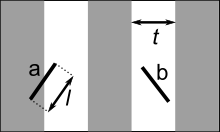
\includegraphics[scale=0.8]{buffon_needle.png}
		\caption{La aguja de Buffon}
		\label{fig:AgujaBuffon}
	\end{figure}
	
	\paragraph{}	
	Los sistemas de simulación de transporte hicieron su aparición hace cuarenta años y la simulación por ordenador comenzó cuando D.L. Gerlough publicó su discurso: \emph{Simulation of freeway traffic on a general-purpose discrete variable computer} (Simulación del tráfico de la autopista en un ordenador de propósito general de variables discretas.) en la Universidad de California, Los Ángeles, en 1955 \cite{Kallberg1971}.
	
	\paragraph{}
	Desde entonces, la simulación por ordenador se ha convertido en una herramienta ampliamente utilizada en la ingeniería del transporte con muchas aplicaciones que van desde la investigación científica hasta la planificación y el entrenamiento.
	
	% Principales líneas de investigación
	
	\paragraph{}
	Actualmente, las líneas de investigación que se están siguiendo en este campo son mayoritariamente simulaciones microscópicas aunque también hay novedades muy interesantes en los modelos teóricos macroscópicos.
	
	% Ejemplo
	
	\paragraph{}
	Como ejemplo de simulador de tráfico podemos nombrar \emph{CORSIM}, el cual permite representar en dos dimensiones una red viaria y simular el flujo del tráfico a lo largo del tiempo indicando una serie de parámetros.
	
	% Integración en el proyecto
	
	\paragraph{}
	En el proyecto que nos ocupa, se va a elaborar un simulador de tráfico microscópico en tres dimensiones que permitirá analizar distintos tipos de configuraciones en una porción limitada de una red viaria.

\newpage

\section{Representación de redes viarias}

	\paragraph{}
	Como se explica en el libro \emph{Fundamentals of Traffic Simulation} \cite{Barcelo2010}, la representación de mapas o de las redes viarias dependerá del tipo de análisis que se quiera llevar a cabo sobre el sistema de transporte.
	
	\paragraph{}
	Inicialmente, la estructura más sencilla para representar lógicamente un mapa será un grafo dirigido, cuyos nodos serán las intersecciones y cuyos arcos serán las secciones viarias que conectan dichas intersecciones, indicando la dirección de las mismas.
	
	\paragraph{}
	Para completar este modelo, se caracterizan los arcos del grafo con atributos como, por ejemplo,  \emph{capacidad del enlace, número de carriles, modos de transporte que pueden utilizar cada carril (bus, coche, taxi, etc), densidad del tráfico, etc.}
	
	\paragraph{}
	Este modelo sencillo puede ser detallado añadiendo nodos para indicar los posibles giros permitidos en una intersección, tal y como se muestra en la figura \ref{fig:RepresentacionMapas1}.
	
	\begin{figure}[ht]
		\centering
			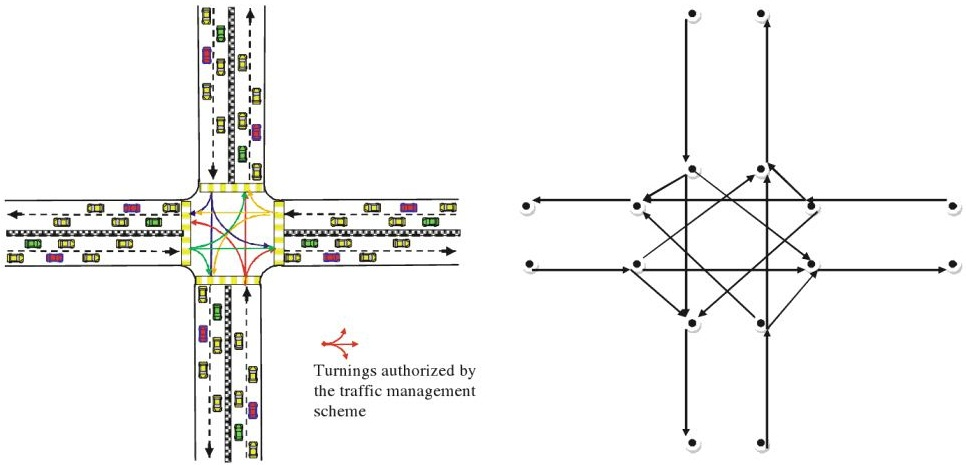
\includegraphics[scale=0.4]{RepresentacionMapas1.jpg}
		\caption{Representación de una intersección (Barceló 2010) \cite{Barcelo2010}}
		\label{fig:RepresentacionMapas1}
	\end{figure}	

	\paragraph{}
	Una vez que tenemos un modelo sencillo, al cual se le pueden añadir tantos detalles como deseemos en forma de atributos en los nodos y en los arcos, se nos presenta el problema de la búsqueda de caminos en una red viaria.
	
	\paragraph{}
	Como solución a dicho problema aparece el estudio \emph{A new data structure to represent road networks} \cite{Bogaert}, en el cual se propone utilizar tres niveles de detalle para representar el mapa. Estos niveles pueden observarse en la figura \ref{fig:RepresentacionMapas2} y en la tabla \ref{table:TablaNiveles}
	
	\begin{figure}[ht]
		\centering
			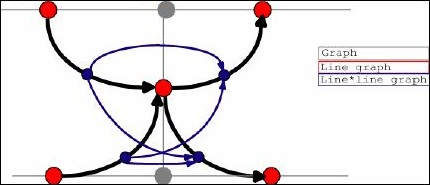
\includegraphics[scale=0.8]{RepresentacionMapas2.jpg}
		\caption{Representación de una intersección (Bogaert) \cite{Bogaert}}
		\label{fig:RepresentacionMapas2}
	\end{figure}
	
	\begin{table}[ht]
		\begin{tabular}{|c|c|c|}
			\hline
			Nivel & Nodos & Arcos \\
			\hline
			\hline
			0 (un grafo) & Intersecciones & Segmentos de vía \\
			\hline
			1 (grafo de líneas) & Segmentos de vía & Giros \\
			\hline
			2 (grafo de líneas de líneas) & Giros & Conexiones entre giros \\
			\hline
		\end{tabular}

	\caption{Niveles representados en la figura \ref{fig:RepresentacionMapas2}}
	\label{table:TablaNiveles}
	\end{table}
	
\section{Sistemas de partículas conductistas}
	
	\paragraph{}
	Los sistemas de partículas son colecciones de objetos independientes, a menudo representados por una sola forma o punto. Todas las partículas tienen una serie de atributos los cuales permiten tener distintos tipos de partícula, tanto en aspecto como en comportamiento.
	
	\paragraph{}
	Generalmente, la implementación de sistemas de partículas conductictas se lleva a cabo mediante la utilización de máquinas de estados finitos, las cuales sirven para modelar el comportamiento de las partículas, de manera que éstas actuarán de una forma u otra en base a sus atributos.
	
	\paragraph{}
	En el caso particular de este proyecto, cada vehículo será una partícula con una serie de características o atributos, lo que nos permitirá modelar distintos tipos de vehículo y distintos tipos de comportamiento de los conductores, con el fin de representar la variedad de los mismos que podemos observar en la realidad.

\section{Modelos de redes viarias reales a partir de imágenes}

	\paragraph{}
	La obtención de redes viarias a partir de imágenes de satélite es un campo de investigación muy importante debido a la gran cantidad de aplicaciones en las que se puede utilizar (militares, civiles, científicas, etc).
	
	\paragraph{}
	El problema consiste en detectar en una imagen, qué es una carretera (camino o vía) y qué no lo es, de forma que esta información pueda ser extraída y procesada.
	
	\paragraph{}
	En el artículo \emph{Road network extraction and intersection detection from aerial images by tracking road footprints} \cite{JiuxiangHu2007} se describe un método de extracción de redes viarias que proporciona muy buenos resultados.
	
	\paragraph{}
	Este método consta de tres pasos:
	\begin{enumerate}	
	\item \emph{Automatic road seeding}: Se analiza el vecindario de todos los píxeles de la imagen y se decide si el pixel es un punto de inicio válido para un segmento de carretera.
	\item \emph{Road tracking}: Comenzando a partir de todas las semillas, se extienden los segmentos de carretera, iterativamente, en una, dos o más direcciones. Se analizan iterativamente el vecindario local de todos los puntos activos en la red viaria para decidir si parar, continuar en una dirección, o dividir en dos o tres direcciones. Este algoritmo va creando un árbol de carreteras.
	\item \emph{Road tree prunning}: Los pasos previos producen una red viaria que contiene casi todos los segmentos de carretera, pero sufre de sobreextracción y pérdidas. Los autores del artículo utilizan una regla de decisión bayesiana para eliminar trozos de la red extraída que parezcan no ser carreteras.
	\end{enumerate}
	
	\paragraph{}
	La inclusión de este método en el proyecto posibilitaría incluir redes viarias reales a la simulación, lo que permitiría probar distintas soluciones de ordenación viaria en entornos reales.

\section{Herramientas gráficas}

	\paragraph{}
	

\chapter{Propuesta}
	\paragraph{}
	En este capítulo expondremos el trabajo que se pretende realizar para conseguir cada uno de los objetivos mostrados en el capítulo anterior.
	
\section{Objetivo principal del proyecto}

	\paragraph{}
	Se desarrollará una aplicación gráfica multiplataforma, mediante la herramienta \emph{Unity3D} utilizando el motor gráfico que incluye, para alojar el simulador de tráfico.
	
	\paragraph{}
	Debido a problemas con Unity3D en la generación de la aplicación para sistemas Linux y a la imposibilidad de realizar pruebas sobre el sistema operativo de Apple, la aplicación será finalmente construida para el sistema operativo Windows en sus versiones de 32 y 64 bits.

\section{Red viaria}
\label{section:RedViaria}
	\paragraph{}
	La red viaria que utilizará el simulador vendrá especificada en un fichero con formato GraphML \cite{GraphML_man}. Dicha red estará determinada por dos grafos, un grafo no dirigido, de topología, en el que los cruces, las curvas y los nodos límite (los puntos de entrada/salida de vehículos desde y hacia la porción de red viaria simulada) serán los nodos, y las vías serán los arcos; y un grafo dirigido, para indicar los giros, en el que los carrilles de las vías serán los nodos y los giros serán los arcos.
	
	\paragraph{}	
	Debido a las restricciones que impone la definición de GraphML sobre los identificadores, cada grafo deberá estar en un fichero distinto. Para ello usaremos dos ficheros por cada red viaria, siendo los ficheros *.topology.graphml para el primer tipo de grafo y los ficheros *.turns.graphml para el segundo. El identificador del grafo en cada uno de los ficheros de la pareja de cada grafo será el mismo.
	
	\paragraph{Nodos del grafo de topología}
	
	\paragraph{}
	Debemos distinguir tres tipos:
	\begin{itemize}
		\item \underline{Nodos de cruce}: Representan un cruce de vías típico. El grado de estos nodos es tres o cuatro.
		
		\begin{figure}[H]
			\centering
				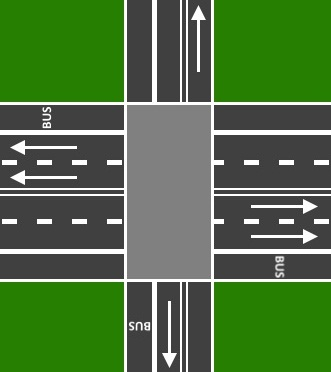
\includegraphics[keepaspectratio,height=100px]{Nodo_cruce.jpg}
		\end{figure}
	
		\item \underline{Nodos de límite de vía}: Representan el límite del área simulada en esa vía. Será el lugar por el que los vehículos salgan y entren desde y hacia la porción de red viaria simulada. El grado de este tipo de nodo es igual a uno. En el entorno 3D tendrán apariencia de tunel.
		
		\begin{figure}[H]
			\centering
				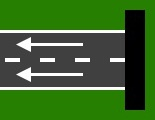
\includegraphics[keepaspectratio,height=50px]{Nodo_limite.jpg}
		\end{figure}
	
		\item \underline{Nodos de continuación}: Representan ángulos en las vías de tal forma que en ellos no se producirán intersecciones de vías. El grado de este tipo de nodo es igual a dos.
		
		\begin{figure}[H]
			\centering
				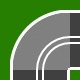
\includegraphics[keepaspectratio,height=50px]{Nodo_continuacion.jpg}
		\end{figure}
	
	\end{itemize}
	
	\paragraph{}
	Por tanto, cada nodo estará definido por un identificador alfanumérico, el tipo de nodo (0: nodo de cruce, 1: nodo de límite de vía, 2: nodo de continuación), sus coordenadas en el plano bidimensional x,y, y para los nodos de tipo cruce, el tipo de cruce, cruce normal (0) o rotonda (1). Las rotondas se han quedado como punto de ampliación de la aplicación.
	\newpage
	\paragraph{Arcos del grafo de topología}	
	\paragraph{}
	Cada arco estará definido por un identificador alfanumérico, el nodo de origen, el nodo de destino, una cadena de texto para poder dar nombre a la vía, y dos cadenas de texto que servirán para indicar los tipos de carril en cada sentido.
	
	\paragraph{}
	Cada una de las cadenas de tipo de carril especificará el tipo de carril o carriles de ese sentido que haya desde el exterior de la vía hacia el interior de la misma utilizando los códigos: P: para indicar un carril de transporte público, N: un carril normal, o la cadena `0' para indicar que no hay carriles en ese sentido.
	
	\paragraph{Nodos del grafo de giros}
	
	\paragraph{}
	Cada nodo estará definido por un identificador alfanumérico que se corresponderá con uno de los identificadores de los carriles de los arcos del grafo de topología. Los identificadores de los carriles tendrán la forma siguiente: identificador del arco al que pertenece, guión bajo, la cadena ``src\_des" o la cadena ``des\_src" en función de la dirección en la que va el carril, (desde el origen al destino o viceversa), guión bajo, número de carril desde el exterior del arco hacia el interior, siendo 0 el primer carril.
	\paragraph{}
	Por ejemplo, el segundo carril del arco ``a2" en dirección origen destino será:
	\begin{lstlisting}
		<node id="a2_src_des_1"/>
	\end{lstlisting}
	
	\paragraph{Arcos del grafo de giros}
	
	\paragraph{}
	Cada arco estará definido por un identificador alfanumérico, el nodo de origen y el nodo de destino. Si el arco está definido significa que el giro está permitido. En el caso de carriles que lleguen a nodos de tipo continuación o límite, no será necesario definir los arcos.
	
	\paragraph{Ejemplo}
	Para ilustrar esta especificación vamos a ver un ejemplo de red viaria y cuál sería su representación en GraphML.
	
	\begin{figure}[H]
		\centering
			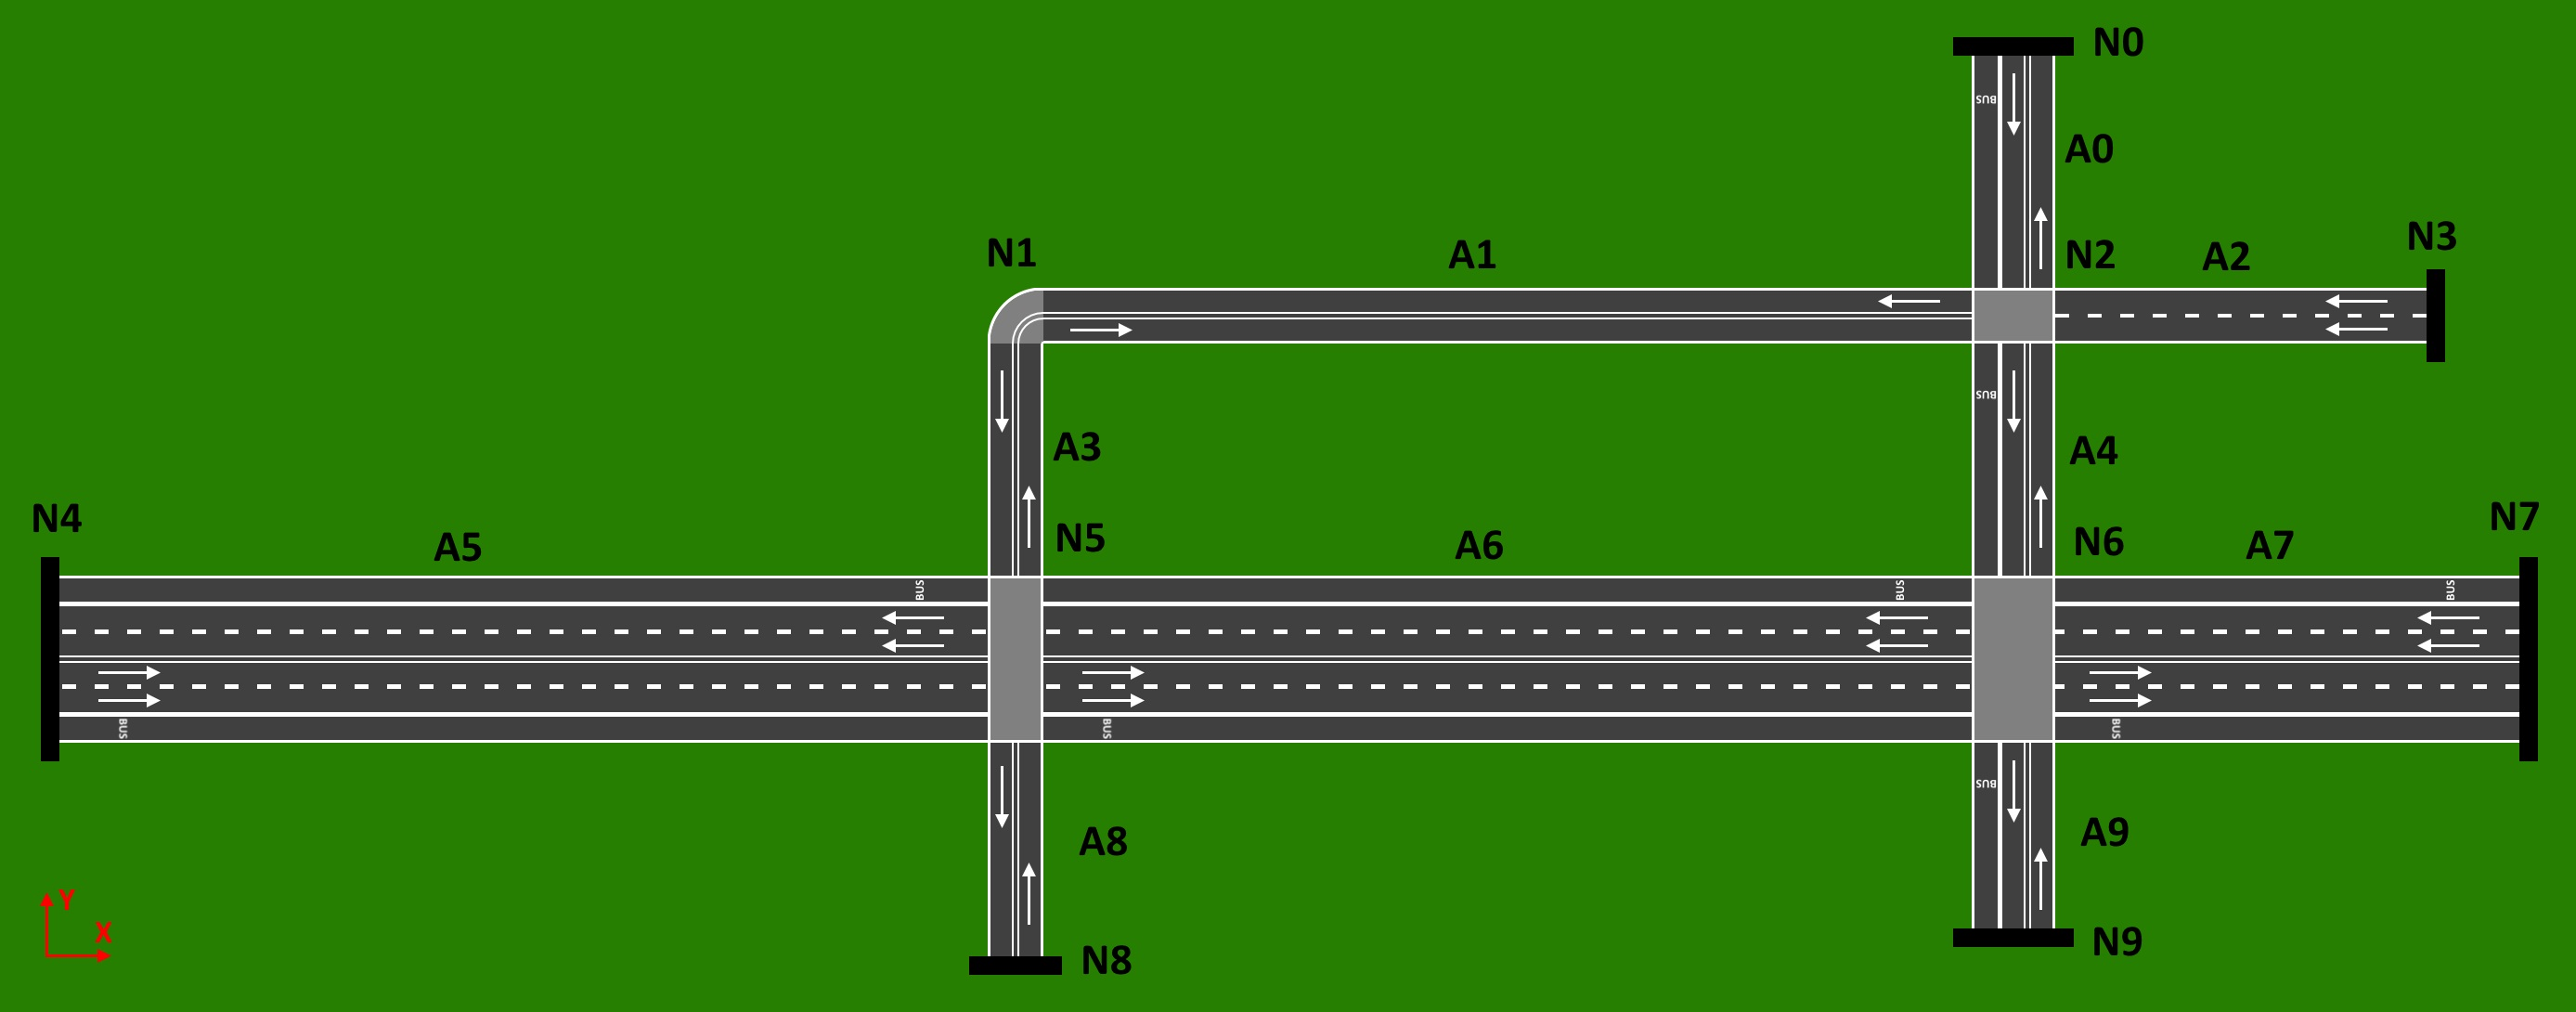
\includegraphics[keepaspectratio,width=359px]{Ejemplo_red_vial.jpg}
	\end{figure}
	
	\paragraph{}
	Como se puede apreciar en la imagen, el grafo de topología asociado consta de diez nodos, tres nodos de tipo cruce, un nodo de tipo continuación y seis nodos de tipo límite de vía. Además, el grafo cuenta con diez arcos que representan las vías de la imagen.
	
	\paragraph{}
	Para este ejemplo se ha supuesto que en cada cruce se puede ir en todas las direcciones que admite esta red, aunque se aprovecha la multiplicidad de carriles para hacer los giros a izquierda desde el carril o carriles situado/s más a la izquierda, y análogamente con los giros a la derecha.
	
	\paragraph{}
	El grafo de giros está compuesto por diez nodos, los arcos del grafo de topología, que en este ejemplo están todos presentes en el grafo debido a que todos están unidos a algún nodo de tipo cruce; y treinta y tres arcos que representan los giros.
	
	\paragraph{}
	A continuación se mostrará la representación de la red viaria con sintaxis de GraphML.
	
	\paragraph{}
	Grafo de topología:
	\tiny
	\lstinputlisting{"../Traffic Flow Simulator/Assets/StreamingAssets/Maps/example_1.topology.graphml"}
	\normalsize
	\paragraph{}	
	Grafo de giros:
	\tiny
	\lstinputlisting{"../Traffic Flow Simulator/Assets/StreamingAssets/Maps/example_1.turns.graphml"}
	\normalsize
	
\section{Señales de tráfico}
\label{section:trafficSignals}
	\paragraph{}
	Como se mencionó anteriormente, las señales con las que cuenta el simulador son semáforos de tres estados. Estos semáforos han sido modelados por mi en Blender \cite{Blender_web} e importados en Unity3D.
	
	\begin{figure}[H]
		\centering
			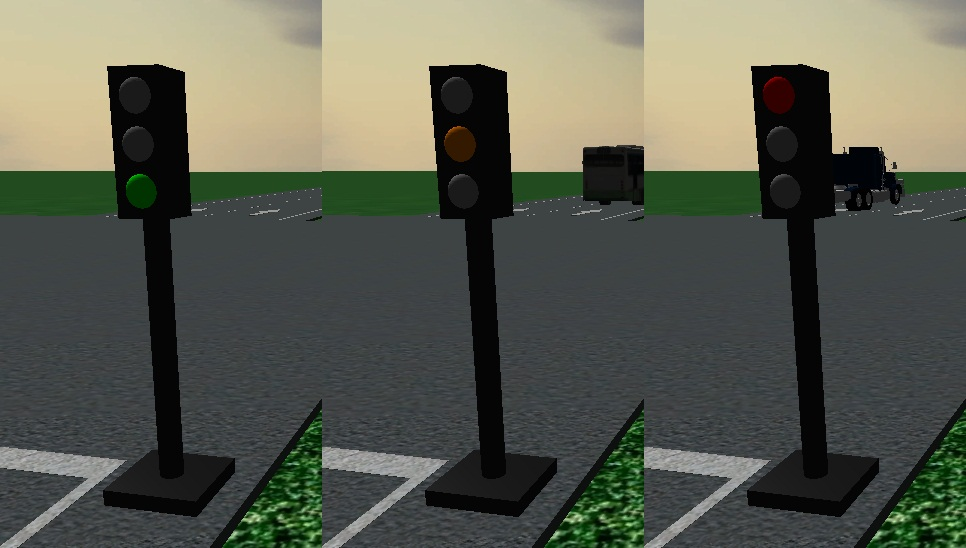
\includegraphics[keepaspectratio,height=150px]{TrafficLightThreeState.jpg}
	\end{figure}
	
	Su funcionamiento consiste en realizar un ciclo contínuo desde el estado rojo, pasando después a verde, luego a naranja y, finalmente, a rojo de nuevo.
	
	\paragraph{}	
	El tiempo que tardan en ponerse en verde por primera vez vendrá determinado por el número de semáforos que haya en un cruce. Se decide aleatoriamente el orden en el que se pondrán en verde y a partir de ahí se calcula el tiempo de retardo para comenzar el ciclo de tal forma que cada semáforo del cruce permanecerá en rojo el tiempo que los demás semáforos utilizan para sus estados verde y naranja.

\section{Vehículos}
	
	\paragraph{}
	Se importarán los siguientes modelos utilizando la herramienta Blender \cite{Blender_web} o el propio importador de modelos obj de Unity3D:
	\begin{itemize}
		\item Bus
		\item Taxi Checker Marathon
		\item Chevrolet Camaro
		\item Todoterreno verde
		\item Todoterreno naranja
		\item Cabeza tractora camión
	\end{itemize}
	
	\paragraph{}	
	Estos modelos no han sido realizados por mi, han sido tomados de lugares con las licencias adecuadas.
	
	\paragraph{}
	Una vez cargados en Unity3D se han ajustado sus escalas en el editor de forma que respetasen en la medida de lo posible las proporciones en las medidas entre unos vehículos y otros.
	
\section{Conductores}
\label{section:driverBehaviour}
	\paragraph{}
	Para simular la lógica de los conductores se ha utilizado un modelo muy básico fundamentándose en tres tipos de conductor:
	
	\begin{itemize}
	\item Buenos
	\item Regulares
	\item Malos
	\end{itemize}
	
	Los buenos conductores respetan la señalización de los semáforos en todo momento, los conductores regulares la respetan con una probabilidad del 50\%, mientras que los malos conductores no respetarán dicha regulación en ningún momento.
	
\section{Entorno}

	\paragraph{}
	El entorno está formado por un suelo con textura de hierba y un skybox para formar el cielo. Los nodos límite son falsos túneles modelados por mi en Blender \cite{Blender_web} e importados en Unity3D.
	\paragraph{}
	Los distintos elementos que conforman las vías de la red han sido modelados en base a cubos escalados dada la complicación para dibujar texturas dentro de otras texturas y así obtener un único plano con la vía representada.
	
\section{Funcionamiento de la aplicación}
	
	\subsection{Menú principal}
	\paragraph{}
	Una vez iniciada la aplicación y pasada la splash screen de Unity3D (estamos usando la versión gratuita de la herramienta) llegamos al menú principal:
	
	\begin{figure}[H]
		\centering
			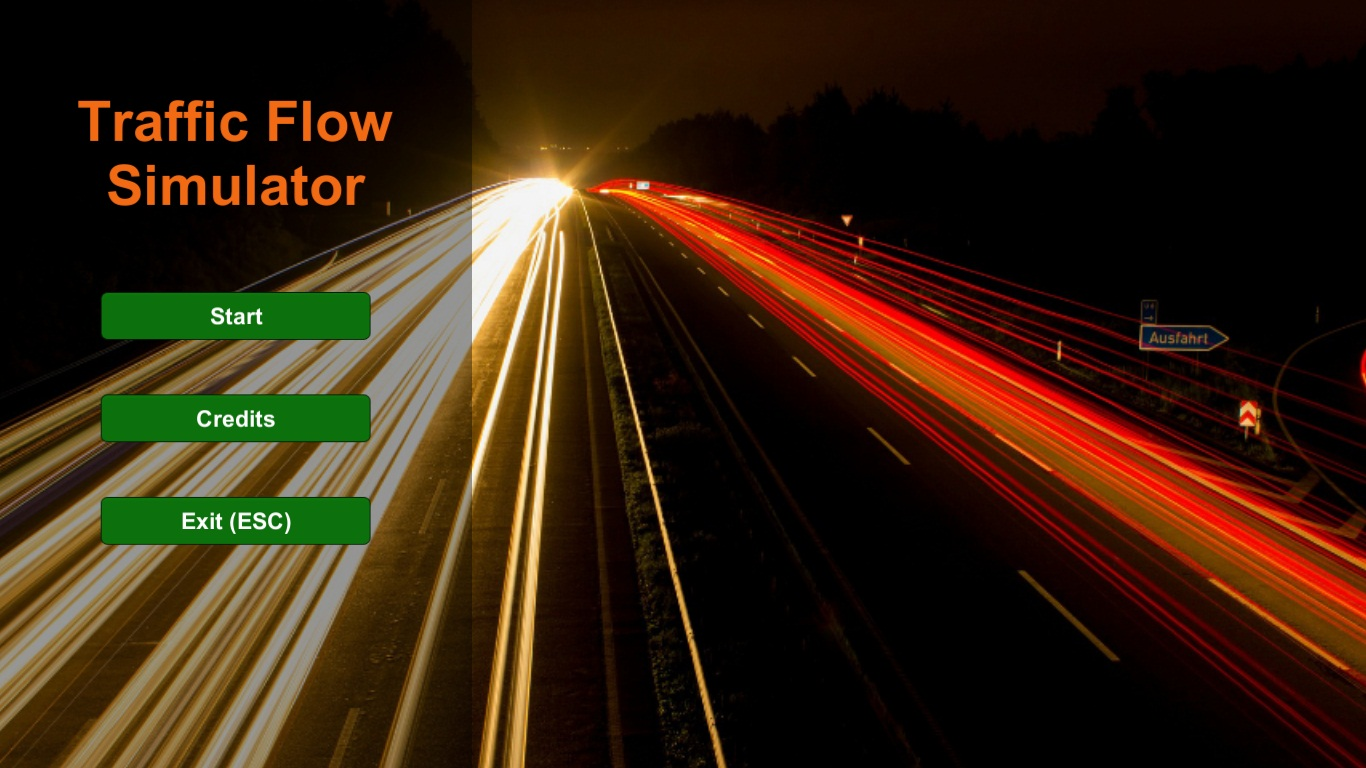
\includegraphics[keepaspectratio,height=150px]{MainMenu.jpg}
	\end{figure}
	
	\paragraph{}
	Desde aquí podemos cargar algún mapa (Start), ver información de la aplicación (Credits) o salir (Exit).

	\paragraph{}	
	Cuando vamos a cargar un mapa, la aplicación lee los nombres de los ficheros, que se encuentran en la carpeta
	\begin{verbatim} "Traffic-Flow-Simulator__x86_Data\StreamingAssets\Maps" \end{verbatim} en el caso de la aplicación para Windows 32 bits o 				\begin{verbatim} "Traffic-Flow-Simulator__x86_64_Data\StreamingAssets\Maps" \end{verbatim} en el caso de la aplicación para Windows 64 bits, y muestra tantos botones como mapas haya, con sus respectivos nombres. Una vez que se pulsa alguno de ellos comienza el proceso de carga y creación de la pantalla de simulación.
	
	\subsection{Pantalla de simulación}
	\paragraph{}
	Al cargar la pantalla de simulación, tanto el skybox como los controles de la Interfaz de Usuario ya están preparados, a continuación se creará el suelo con las dimensiones del mapa cargado más un margen, se representará la red viaria, se posicionará la cámara y dará comienzo la simulación con la creación de vehículos.
	
	\subsection{Representación de los arcos}
	\paragraph{}
	La representación de la red viaria comienza con el dibujado de los arcos del grafo (los tramos rectos de red viaria) que se dibujan de la siguiente forma:
	
	% Explicación del dibujado de los arcos
	\paragraph{}
	Se comienza con una plataforma viaria escalada en el eje Z de forma que el nodo origen del arco se encuentre hacia la parte negativa del eje Z y el nodo destino hacia la parte positiva del eje Z. A continuación se dibujan las líneas de los arcenes. Seguidamente, si el arco tiene carriles en ambas direcciones se dibujan las líneas de mediana (líneas centrales de división de sentidos), atendiendo a que éstas verán modificada su posición desde el centro del arco en función de la diferencia del número de carriles que haya en cada sentido.
	\paragraph{}
	A continuación, para cada uno de los sentidos en el que haya carriles, se dibujarán tantas líneas de carril como carriles haya en dicho sentido menos una, desde el exterior del arco hacia el centro, atendiendo al tipo de carril que le haya sido asignado, así, un carril taxi bus será delimitado por la izquierda por una línea contínua ancha mientras que los carriles normales serán delimitados por la izquierda por líneas discontínuas estrechas.
	\paragraph{}
	Para finalizar el dibujado de líneas, si los carriles del sentido que se está dibujando llegan a un nodo de intersección, se dibujará una línea de detención perpendicular a las anteriores.
	\paragraph{}
	Además, al comienzo de cada carril se dibujarán marcas horizontales que indicarán el tipo de carril: siendo la flecha blanca para los carriles normales y las letras TAXI BUS para los carriles de tipo público.
	\paragraph{}
	Por último, se añadirán los semáforos al final del arco en el arcén de cada sentido si se desemboca en un cruce, orientados adecuadamente según el sentido que se esté dibujando.
	\paragraph{}
	A continuación podemos ver una imagen que ilustra la explicación anterior:
	
	\begin{figure}[H]
		\centering
			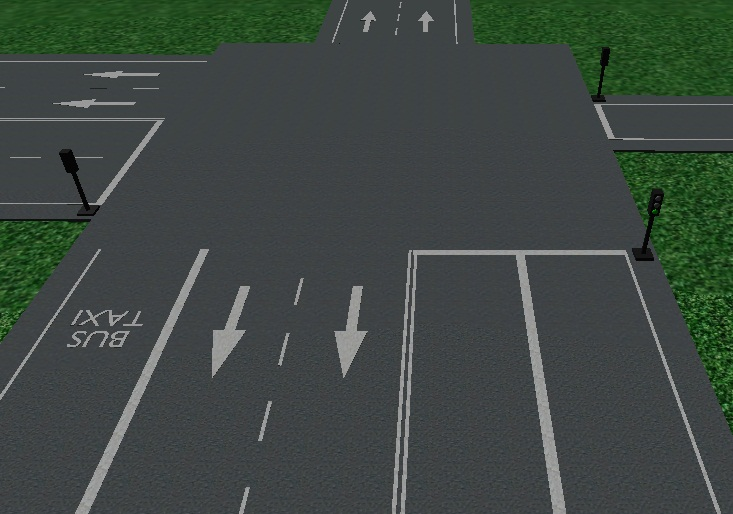
\includegraphics[keepaspectratio,height=150px]{BuildEdgeExample.jpg}
	\end{figure}
	
	\paragraph{}
	Una vez que la representación del arco ha sido construida se coloca en su posición y se orienta para quedar alineada con los nodos origen y destino. La posición no será el punto medio de las posiciones de los nodos ya que según el tipo de nodo que se encuentre en el extremo habrá que realizar un pequeño ajuste de posición. Además la longitud del arco tampoco será la distancia entre los nodos ya que entonces se solaparían las representaciones, esta ha sido calculada de forma que no solape en ninguno de los dos extremos con las representaciones de los nodos.
	
	\paragraph{}
	Además, para el guiado de los vehículos, los arcos contarán con nodos guía (invisibles en la aplicación) al principio y final de cada carril, así como dos nodos guía en el centro que servirán para hacer cambios de carril si los carriles contiguos son del mismo tipo. Veamos un ejemplo:
	
	\begin{figure}[H]
		\centering
			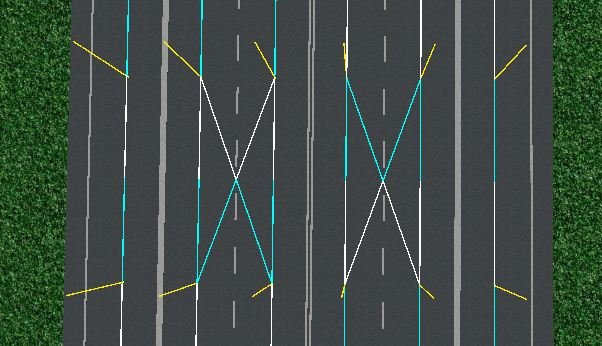
\includegraphics[keepaspectratio,height=150px]{laneCross.jpg}
	\end{figure}
	
	\paragraph{}
	Como se puede apreciar en la imagen, los carriles más exteriores no permiten cambio de carril dado que son de tipo público y no hay más carriles de tipo público contiguos a ellos, mientras que los demás si permiten el cambio ya que son contiguos de tipo normal.
	
	\subsection{Representación de los nodos}
	\paragraph{}
	A continuación se dibujan los nodos. Según su tipo, serán dibujados de la siguiente forma:
	
	\begin{itemize}
	\item Nodos límite:
	% Explicación del dibujado de los nodos límite
	\newline
	La representación de los nodos límite es la más sencilla que podemos encontrar, consiste en instanciar un tunel 3D en la posición del nodo límite, escalarlo a lo ancho para abarcar todo el ancho del arco que llega hasta él y rotarlo de manera que quede alineado con dicho arco.
	\newline
	\newline
	Este tipo de nodo no afecta en manera alguna la circulación de los vehículos, por tanto, los vehículos se introducirán en el tunel y desaparecerán al llegar al nodo guía de final de carril por no tener ningún nodo guía siguiente.
	
	\begin{figure}[H]
		\centering
			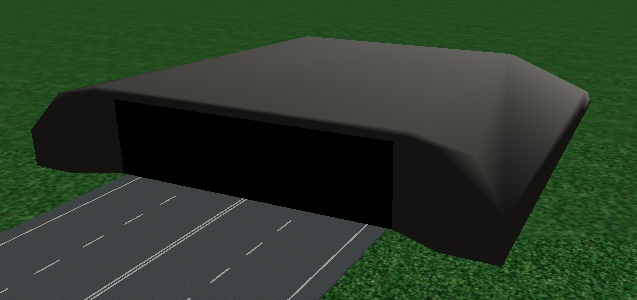
\includegraphics[keepaspectratio,height=150px]{tunnel.jpg}
	\end{figure}
	
	\item Nodos de intersección:
	% Explicación del dibujado de los nodos de intersección
	\newline
	Para representar un nodo de intersección se toma una plataforma viaria vacía, es decir sin líneas ni marcas, se instancia en la posición correspondiente y se escala de tal forma que quede una forma completamente cuadrada cuyos laterales tienen la misma dimensión que la anchura del arco más ancho de los que inciden en dicho nodo.
	\newline
	\newline
	Además, para el guiado de los vehículos, el nodo de intersección une los nodos guía de final de carril con los de inicio de carril según los giros permitidos indicados en el fichero de giros explicado en la sección \emph{\ref{section:RedViaria} \nameref{section:RedViaria}}. Para ello, traza una curva de Bézier \cite{BezierCurves} con nodos guía intermedios por cada uno de los giros permitidos.
	
	\begin{figure}[H]
		\centering
			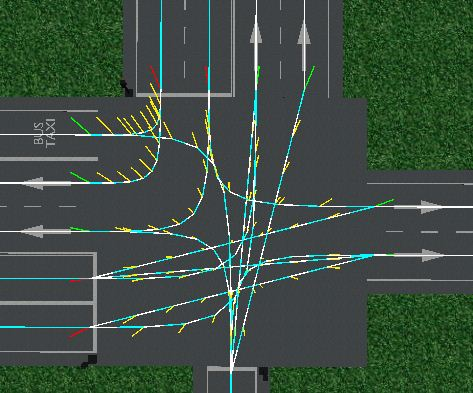
\includegraphics[keepaspectratio,height=200px]{IntersectionGuideNodes.jpg}
	\end{figure}
	
	\item Nodos de continuación:
	\newline
	\newline
	% Explicación del dibujado de los nodos de continuación
	Los nodos de continuación (tramos curvos) se dibujan de forma análoga a los arcos, con un par de excepciones: en estos nodos no se permite el cambio de carril y en vez de ser una plataforma recta son diez tramos de plataforma con sus líneas correspondientes que conforman la forma curva.
	\newline
	\newline
	Para conseguir la forma curva se ha utilizado una curva de Bézier \cite{BezierCurves} con tres puntos, el punto central de la curva en el extremo del arco de referencia, el punto central de la curva en el extremo del otro arco que incide en el nodo y el punto central en el que se cruzarían los arcos. Este último punto se utiliza como los dos puntos de control propios de una curva de Bézier \cite{BezierCurves}.
	\newline
	\newline
	Además, se incluyen nodos de guiado intermedios para que los vehículos simulen el giro a lo largo de la sección curva. Finalmente se coloca en la posición adecuada y se alinea con los arcos que inciden en el nodo, como se puede apreciar en la siguiente imagen:
	
	\begin{figure}[H]
		\centering
			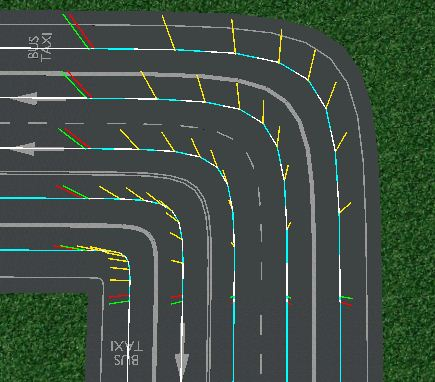
\includegraphics[keepaspectratio,height=200px]{ContinuationNodeGuideNodes.jpg}
	\end{figure}
	
	\end{itemize}
	
	\subsection{Finalizando la representación}
	\paragraph{}
	Como paso final, se unen los nodos guía de final de carril de los arcos con los nodos correspondientes de los nodos de continuación e intersección.
	
	\paragraph{}
	Una vez representada toda la red viaria se sincronizan los semáforos tal y como se explicó en el apartado \emph{\ref{section:trafficSignals} \nameref{section:trafficSignals}}.
	
	\paragraph{}
	Así concluye la representación de la red viaria, a continuación, da comienzo la simulación generando los vehículos atendiendo a los parámetros de la interfaz de usuario.
	
	\paragraph{}
	Dicha interfaz pondrá a disposición del usuario unos controles deslizantes (sliders) para controlar las siguientes variables:
	
	\begin{itemize}
	\item El número de vehículos dentro de la simulación, con un mínimo de 0 y un máximo de 200.
	\item La proporción de cada tipo de conductor, bueno, regular y malo, con un mínimo de 0\% y un máximo de 100\%, respetándose un total entre los tres tipos del 100\%.
	\item La proporción de cada tipo de vehículo, público y privado, con un mínimo de 0\% y un máximo de 100\%, respetándose un total entre los dos tipos del 100\%.
	\item El tiempo que pasan los semáforos en verde, con un mínimo de 5 segundos y un máximo de 60 segundos.
	\item El tiempo que tardan en eliminarse de la simulación los vehículos accidentados, con un mínimo de 0 segundos y un máximo de 180 segundos.
	\end{itemize}
	
	\paragraph{}
	Así mismo, la interfaz también dispone de un contador de vehículos accidentados, un botón para pausar/reanudar la simulación o volver al menú principal, un botón para mostrar el panel de ayuda con la información relativa a los controles de la cámara y un botón para mostrar/ocultar los nombres de las calles.
	
	\subsection{Comportamiento de los vehículos}
	\paragraph{}
	Cada vehículo es instanciado en un nodo guía, dentro de un túnel, y se le asigna como objetivo que se desplace al siguiente nodo guía, cuando llega a este, comprueba a cuántos nodos guía puede avanzar atendiendo al tipo de vehículo que puede circular por cada nodo y elige uno de forma aleatoria, repitiendo este ciclo de forma indefinida hasta que llega a un nodo el cual no tiene nodos guía siguientes, lo cual significa que el vehículo se encuentra dentro de un tunel y que debe eliminarse de la simulación. Esto provocará una actualización automática de los contadores de cantidad de vehículos, tipo de vehículos y tipos de conductor, de cara a la instanciación de nuevos vehículos.
	
	\paragraph{}
	Cada vehículo va comprobando constantemente que no haya vehículos en su camino a una distancia inferior a diez metros, en cuyo caso moderará su velocidad para no chocar con el vehículo que tenga inmediatamente delante. Para ello comprueba si existe alguno entre su posición y su nodo guía objetivo, si no hay ninguno y aún no ha comprobado los diez metros, comprobará de forma recursiva desde el nodo guía objetivo hasta cualquiera de los siguientes, y así sucesivamente.
	
	\paragraph{}
	Además, cada vehículo cuenta con dos rayos, para raycasting, de metro y medio en la parte frontal orientados hacia delante y hacia los lados para comprobar que no hay vehículos en las inmediaciones por delante; así como un rayo más en la parte frontal de 10 metros para la detección de los semáforos.
	
	\paragraph{}
	Si un vehículo detecta un semáforo en verde no hará ningún cambio, mientras que si lo detecta en naranja o rojo disminuirá la velocidad hasta detenerse cerca de la línea de detención. Esto ocurrirá para los buenos conductores, ya que, como se mencionó en el apartado \emph{\ref{section:driverBehaviour} \nameref{section:driverBehaviour}}, los malos conductores no lo harán y los conductores regulares se lo pensarán constantemente mientras se acercan al semáforo, ya que en cada frame realizan una evaluación de la situación, pudiendose casi detener y luego reanudar la marcha con el semáforo en un estado distinto al verde.

\bibliographystyle{ieeetr}
\bibliography{bibProyecto}

\end{document}
